\documentclass[../main.tex]{subfiles}
\begin{document}
% \section{Macros pour tracer des tangentes }
\section{绘制切线}

% Si une seule fonction est utilisée, elle est stockée avec comme nom
% \tkzcname{tkzFcta}, si une deuxième fonction est utilisée, elle sera stockée avec comme nom \tkzcname{tkzFctb}, et ainsi de suite\ldots Si plusieurs fonctions sont présentent dans un même environnement alors l'option \tkzname{with} permet de choisir celle qui sera mise à contribution.
需要说明的是,在使用\tkzcname{tkzFct}命令定义函数后,
对第1个函数命名为\tkzcname{tkzFcta},第2个函数命名为\tkzcname{tkzFctb},以此类推\ldots。
如果一个环境中有多个函数,则可以使用\tkzname{with}指定需要使用的函数。

\tkzHandBomb 在使用\tkzcname{tkzFct}命令和\tkzcname{tkzDrawTangentLine}命令之前,
需要使用\tkzcname{tkzInit}命令初始化绘图环境。
可以用\tkzname{kl}和\tkzname{kr}系数指定半切线矢量长度,
如$kl=0$或$kr=0$表示取消对应的半切线(l=left,r=right)。
如果\tkzname{xstep=1}和\tkzname{ystep=1},斜率为1,则半切线的长度是$\sqrt{2}$。
其他情况下,如果半切线向量$\vec{AT}$的斜率是$p$,则半切线向量是(\tkzname{kl},\tkzname{kl*p})。


% \subsection{Représentation d'une tangente \tkzcname{tkzDrawTangentLine}}
\subsection{\tkzcname{tkzDrawTangentLine}命令:绘制切线}
\hypertarget{tdtl}{}
% \begin{NewMacroBox}{tkzDrawTangentLine}{\oarg{命令选项}\parg{a}}
% \emph{On l'emploie soit juste après l'utilisation de \tkzcname{tkzFct}, sinon il faut donner la référence de la fonction à l'aide de l'option \tkzname{with}.}
%
% \medskip
% \begin{tabular}{lll}
%  \toprule
%  options             & exemple & explication    \\
%  \midrule
%  \TAline{a}{\tkzcname{tkzDrawTangentLine(0)}}{tangente au point d'abscisse $0$}
%  \bottomrule
% \end{tabular}
%
% Les options sont celles de \TIKZ comme \tkzname{color} ou \tkzname{style} plus les options suivantes
%
% \begin{tabular}{lll}
% \toprule
% options             & défaut & définition                         \\
% \midrule
% \TOline{draw}{false}{booléen si true alors le point de contact est tracé}
% \TOline{with}{a}{permet de choisir une fonction}
% \TOline{kr}{1}{coefficient pour la longueur de la demi-tangente à droite}
% \TOline{kl} {1}{coefficient pour la longueur de la demi-tangente à gauche}
% \end{tabular}
% \end{NewMacroBox}
%<--------------------------------------------------------------------------->
\begin{NewMacroBox}{tkzDrawTangentLine}{\oarg{命令选项}\parg{切点横坐标}}
\emph{
如果直接在\tkzcname{tkzFct}命令后使用该命令,表示使用当前函数。
否则,需要用\tkzname{with}选项指定函数。}

\medskip
\begin{tabular}{lll}
 \toprule
 参数             & 样例 & 说明    \\
 \midrule
 \TAline{切点横坐标}{\tkzcname{tkzDrawTangentLine(0)}}{横坐标为$0$的函数点处的切线}
 \bottomrule
\end{tabular}

可以使用所有类似\tkzname{color}或\tkzname{style}的有效\TIKZ 选项。

\begin{tabular}{lll}
\toprule
选项             & 默认值 & 含义                         \\
\midrule
\TOline{draw}{false}{布尔值,如为true,则绘制切点}
\TOline{with}{a}{选择指定的函数}
\TOline{kr}{1}{右半切线长度系数}
\TOline{kl} {1}{左半切线长度系数}
\end{tabular}
\end{NewMacroBox}
% \subsection{Tangente avec \tkzname{xstep} et \tkzname{ystep} différents de 1}
\subsection{\tkzname{xstep}和\tkzname{ystep}不为1的切线}

\begin{tikzpicture}[xscale=1.5]
 \tikzset{tan style/.style={-}}
 \tkzInit[xmin=0,xmax=800,xstep=100,ymin=0,ymax=1800,ystep=400]
 \tkzGrid[color=brown,sub,subxstep=50,subystep=200](0,0)(800,1800)
 \tkzAxeXY
 \tkzFct[color=red,samples=100,domain = 0:800]%
    {(1./90000)*\x*\x*\x-(1./100)*\x*\x+(113./36)*\x}
 \tkzDrawTangentLine[draw,color=blue,kr=300,kl=450](450)
  \tkzText[draw,color = black,fill = brown!50,opacity  = 0.8](300,1200)%
 {$f(x)=\dfrac{1}{90000}x^3 -\dfrac{1}{{100}}x^2 +\dfrac{113}{36}x$}
 \end{tikzpicture}

% Il faut remarquer qu'il n'est point nécessaire  de faire des calculs. Il suffit d'utiliser les valeurs qui correspondent aux graduations.
要说明的是,没有必要计算坐标真实值,只需要直接指定与刻度对应的坐标值即可。

% On peut changer le styavec le des tangentes avec,  par exemple,
例如,可以使用如下类似代码修改切线样式:

\tkzcname{tikzset\{tan style/.style=\{-\}\}} 的默认设置为:

\tkzcname{tikzset\{tan style/.style=\{->,>=latex\}\}}

\begin{tkzexample}[code only]
\begin{tikzpicture}[xscale=1.5]
 \tikzset{tan style/.style={-}}
 \tkzInit[xmin=0,xmax=800,xstep=100,
          ymin=0,ymax=1800,ystep=400]
 \tkzGrid[color=brown,sub,subxstep=50,subystep=200](0,0)(800,1800)
 \tkzAxeXY
 \tkzFct[color=red,samples=100,domain = 0:800]%
    {(1./90000)*\x*\x*\x-(1./100)*\x*\x+(113./36)*\x}
 \tkzDrawTangentLine[color=blue,kr=300,kl=450,coord](450)
 \tkzText[draw, color    = black,%
           fill     = brown!50, opacity  = 0.8](300,1200)%
 {$f(x)=\dfrac{1}{90000}x^3 -\dfrac{1}{{100}}x^2 +\dfrac{113}{36}x$}
 \end{tikzpicture}
 \end{tkzexample}
%<--------------------------------------------------------------------------->
% \subsection{Les options \tkzname{kl}, \tkzname{kr} et l'option \tkzname{draw}}
\subsection{\tkzname{kl}、\tkzname{kr}和\tkzname{draw}选项}
% Si l'un des deux nombres \tkzname{kl} ou \tkzname{kr} est nul alors seulement une demi-tangente est tracée sinon ces nombres représentent un pourcentage de la longueur initiale de la tangente. L'option \tkzname{draw} permet de tracer le point de contact.
如果\tkzname{kl}或\tkzname{kr}为0,则只绘制半切线,否则,可以用数字表示切线长度与切向量长度的百分比。
\tkzname{draw}选项表示需要绘制切点。

\begin{tkzexample}[]
  \begin{tikzpicture}[scale=1.5]
   \tkzInit[xmin=-3,xmax=4,ymin=-4,ymax=2]
   \tkzGrid   \tkzDrawXY \tkzClip
   \tkzFct[domain = -2.15:3.2]{(-x*x)+2*x}
   \tkzDefPointByFct[draw](2)
   \tkzDrawTangentLine[kl=0,draw](-1)
   \tkzDrawTangentLine[draw](1)
   \tkzDrawTangentLine[kr=0,draw](3)
   \tkzRep
 \end{tikzpicture}
\end{tkzexample}

%<–––––––––––––––––––––––––––––––––––––––––––––––––––––––––––––––––––––––––––>
% \subsection{Tangente et l'option \tkzname{with}}
\subsection{\tkzname{with}选项}
% Soit on place la macro  \tkzcname{tkzDrawTangentLine}    après la ligne
%  qui définit la première fonction $(a)$, soit  on trace une autre fonction avant, et dans ce cas, il est nécessaire de préciser quelle fonction sera utilisée. pour se faire, on utilise l'option \tkzname{with}.
可以将\tkzcname{tkzDrawTangentLine}放在第一个函数定义代码行之后,表示使用该函数,
当然,也可以使用\tkzname{with}选项指定需要绘制切线的函数。

\begin{tkzexample}[]
\begin{tikzpicture}[scale=4]
 \tkzInit[xmax=3,ymax=2]
 \tkzAxeXY
 \tkzGrid(0,0)(3,2)
 \tkzFct[color   = red, domain = 1/3:3]{0.125*(3*x-1)+0.375*(3*x-1)/(x*x)}
 \tkzFct[color   = blue, domain = 1/3:3]{0.125*(3*x-1)}
 \tkzDrawTangentLine[with=a,
                     color=blue](1)
 \tkzText[draw,
          color= red](1,1.5)%
          {$f(x)=\frac{1}{8}(3x-1)+\frac{3}{8}\left(\frac{3x-1}{x^2}\right)$}
 \tkzText[draw,
          color= blue](2,0.3)%
          {$g(x)=\frac{1}{8}(3x-1)$}
\end{tikzpicture}
\end{tkzexample}
%<–––––––––––––––––––––––––––––––––––––––––––––––––––––––––––––––––––––––––––>
\subsection{切线示例}

\begin{tkzexample}[]
\begin{tikzpicture}[scale=2]
  \tkzInit[xmin=-5,xmax=2,ymin=-1, ymax=3]
  \tkzDrawX
  \tkzDrawY
  \tkzText[draw,color = red,fill = orange!20]( 1.5,1.5){$y = xe^x$}
  \tkzFct[color = red, domain = -5:1]{x*exp(x)}%
  \tkzDrawTangentLine[color=blue,kr=2,kl=2](-2)
  \tkzDrawTangentLine[color=green,kr=2,kl=2](-1)
  \tkzDrawTangentLine[color=blue](0)
  \tkzDrawTangentLine[color=blue,kr=0](1)
\end{tikzpicture}
\end{tkzexample}
%<–––––––––––––––––––––––––––––––––––––––––––––––––––––––––––––––––––––––––––>
% \subsection{Demi-tangentes }
\subsection{半切线}
% Il faut remarquer que les tangentes sont en réalité deux demi-tangentes ce qui permet d'obtenir simplement le résultat ci-dessous.
注意,切线有两条半切线,例如对于函数:

% Poosible sont les écritures \tkzname{(((x+1)*x)*x)**0.5},   \tkzname{(x**3+x**2)**0.5} et \tkzname{(x*x*x+x*x)**(0.5)}.
\tkzname{(((x+1)*x)*x)**0.5}(\tkzname{(x**3+x**2)**0.5}或\tkzname{(x*x*x+x*x)**(0.5)}).

% Dans cet exemple, les deux demi-tangentes sont obtenues automatiquement :
在本例中,能够自动得到两条半切线。

\begin{tkzexample}[]
 \begin{tikzpicture}[scale=2.75]
     \tkzInit[xmin=-2,xmax=3,ymax=3]
     \tkzGrid[color=orange](-2,0)(3,3)
     \tkzAxeX
     \tkzAxeY
     \tkzFct[color = red ,domain = -1:2]{(((x+1)*x)*x)**0.5}
     \tkzDrawTangentLine(0)
     \tkzText[draw,color = red,fill = orange!20](2,1){$f(x)=\sqrt{x^3+x^2}$}
 \end{tikzpicture}
\end{tkzexample}
%<–––––––––––––––––––––––––––––––––––––––––––––––––––––––––––––––––––––––––––>
% \subsection{Demi-tangentes Courbe de Lorentz }
\subsection{Lorentz曲线的半切线}

% Ici, on ne veut que les demi-tangentes comprises entre 0 et 1, pour cela il suffit dans un cas de donner la valeur 0 à \tkzname{kr} et dans l'autre à \tkzname{kl}.
在此,只需得到0和1之间的半切线,为此,仅需\tkzname{kr}和\tkzname{kl}取合适的值即可。

\begin{center}
\begin{tkzexample}[vbox]
\begin{tikzpicture}[scale=1.25]
  \tkzInit[xmax=1,ymax=1,xstep=0.1,ystep=0.1]
  \tkzGrid(0,0)(1,1)
  \tkzAxeXY
  \tkzFct[color = red,thick, domain =0:1]{(exp(\x)-1)/(exp(1)-1)}
  \tkzSetUpPoint[size=4]
  \tkzDrawTangentLine[draw, kl = 0,  kr = 0.4](0)
  \tkzDrawTangentLine[draw, kl = 0.4,kr = 0  ](1)
  \tkzText[draw,color = red,fill = orange!20](0.5,0.6)%
          {$f(x)=\dfrac{\text{e}^x-1}{\text{e}-1}$}
\end{tikzpicture}
\end{tkzexample}
\end{center}
%<--------------------------------------------------------------------------->
\subsection{切线族示例}


\begin{tkzexample}[vbox]
\begin{tikzpicture}[scale=2]
  \tikzstyle{tan style}=[-]
  \tkzInit[xmin=-5,xmax=2,ymin=-1,ymax=3]
  \tkzDrawXY
  \tkzText[draw,color = red, fill = orange!20](1.5,1.5){$y = xe^x$}
  \tkzFct[line width = 0.01 pt,color = red, domain = -5:1]{x*exp(x)}
  \foreach \x in {-4,-3.8,...,0}{%
    \tkzDrawTangentLine[color=blue,line width=.4pt,kr=1,kl=0.5](\x)}
  \foreach \x in {0.6,0.8,1}{%
     \tkzDrawTangentLine[color=blue,line width=.4pt, kr=0,kl=0.5](\x)}
\end{tikzpicture}
\end{tkzexample}
%<--------------------------------------------------------------------------->
\subsection{无曲线切线族}

% Pour cela, il faut définir la dernière expression avec la syntaxe de \tkzname{fp.sty}.
由于不需要绘制函数曲线,因此不能使用\tkzcname{tkzFct}命令定义函数,
为此,必须使用符合\tkzname{fp.sty}语法的表达式定义函数。

需要定义\tkzcname{tkzFctLast}全局宏以保存函数表达式。

\begin{tkzltxexample}[]
	 \global\edef\tkzFctLast{x*exp(x)}
\end{tkzltxexample}

% \subsubsection{Utilisation de \tkzcname{tkzFctLast}}
\subsubsection{\tkzcname{tkzFctLast}宏}
\begin{tkzexample}[vbox]
\begin{tikzpicture}[scale=2]
  \tikzstyle{tan style}=[-]
  \tkzInit[xmin=-5,xmax=2,ymin=-1,ymax=3]
  \tkzDrawXY
  \tkzText[draw,color = red, fill = orange!20](1.5,1.5){$y = xe^x$}
  \global\edef\tkzFctLast{x*exp(x)}% 这一行代码非常重要
  \foreach \v in {-4,-3.8,...,0}{%
    \tkzDrawTangentLine[color=blue,line width=.4pt,kl=1](\v)}
  \foreach \v in {0.6,0.8,1}{%
    \tkzDrawTangentLine[color=blue,line width=.4pt,kr=0,kl=.75](\v)}
\end{tikzpicture}
\end{tkzexample}


\newpage
\subsection{历史记录}

% Un problème surgit si on emploie une expression contenant des parenthèses dans l'argument, ainsi \tkzname{(\{1/exp(1)\})} est correct  mais \tkzname{(1/exp(1))} donne une erreur. Il est aussi possible d'évaluer l'antécédent postérieurement comme cela~:
如果在参数中使用带有括号的表达式,则会出现问题。
所以,\tkzname{(\{1/exp(1)\})}是正确的,但\tkzname{(1/exp(1))}则会引发错误。
在后续计算中,也需要注意该问题。

\subsubsection{保存计算结果}
\begin{tkzltxexample}[]  \FPeval\vx{1/exp(1)}
\end{tkzltxexample}

\subsubsection{使用计算结果}
\begin{center}
\begin{tkzexample}[]
\begin{tikzpicture}[scale=1]
  \tkzInit[xmax=1,xstep=0.1,ymin=0.5,ymax=1,ystep=0.1]
  \tkzGrid      \tkzAxeXY
  \tkzFct[domain = 0.00001:1]{(\x**\x)}
  \tkzDrawTangentLine[draw,color = red, kr = 0.2,kl = 0.2]({1/exp(1)})
\end{tikzpicture}
\end{tkzexample}
\end{center}



\end{document}
\endinput
